\documentclass[12pt,landscape]{article}
\usepackage{multicol}
\usepackage{calc}
\usepackage{ifthen}
\usepackage{tabulary}
\usepackage[landscape]{geometry}
\usepackage{amsmath,amsthm,amsfonts,amssymb}
\usepackage{color,graphicx,overpic}
\usepackage{hyperref}
\usepackage{soul} %for highlight
\usepackage{xcolor} %color definition
\usepackage{sectsty} %change section color
\graphicspath{ {figures/} } %set figures path


\pdfinfo{
  /Title (EC3102 Macroeconomics cheatsheet)
  /Creator (Lingjie)}

% This sets page margins to .5 inch if using letter paper, and to 1cm
% if using A4 paper. (This probably isn't strictly necessary.)
% If using another size paper, use default 1cm margins.
\ifthenelse{\lengthtest { \paperwidth = 11in}}
    { \geometry{top=.5in,left=.5in,right=.5in,bottom=.5in} }
    {\ifthenelse{ \lengthtest{ \paperwidth = 297mm}}
        {\geometry{top=1cm,left=1cm,right=1cm,bottom=1cm} }
        {\geometry{top=1cm,left=1cm,right=1cm,bottom=1cm} }
    }

% Turn off header and footer
\pagestyle{empty}

% Redefine section commands to use less space
\makeatletter
\renewcommand{\section}{\@startsection{section}{1}{0mm}%
                                {-1ex plus -.5ex minus -.2ex}%
                                {0.5ex plus .2ex}%x
                                {\normalfont\large\bfseries\color{red}}}
\renewcommand{\subsection}{\@startsection{subsection}{2}{0mm}%
                                {-1explus -.5ex minus -.2ex}%
                                {0.5ex plus .2ex}%
                                {\normalfont\normalsize\bfseries\color{blue}}}
\renewcommand{\subsubsection}{\@startsection{subsubsection}{3}{0mm}%
                                {-1ex plus -.5ex minus -.2ex}%
                                {1ex plus .2ex}%
                                {\normalfont\small\bfseries\color{violet}}}
\makeatother

% Define BibTeX command
\def\BibTeX{{\rm B\kern-.05em{\sc i\kern-.025em b}\kern-.08em
    T\kern-.1667em\lower.7ex\hbox{E}\kern-.125emX}}

% Don't print section numbers
\setcounter{secnumdepth}{0}


\setlength{\parindent}{0pt}
\setlength{\parskip}{0pt plus 0.5ex}

%My Environments
\newtheorem{example}[section]{Example}
% -----------------------------------------------------------------------

\begin{document}
\raggedright
\footnotesize
\begin{multicols}{3}


% multicol parameters
% These lengths are set only within the two main columns
%\setlength{\columnseprule}{0.25pt}
\setlength{\premulticols}{1pt}
\setlength{\postmulticols}{1pt}
\setlength{\multicolsep}{1pt}
\setlength{\columnsep}{2pt}

\begin{center}
     \Large{\underline{EC3102 Macroeconomics II}} \\
     {Lingjie, \today}
\end{center}

\section{Infinite-Period Framework}
	\begin{tabular}{ll}
		inflation (real)				&		$\pi_{t+1} = \frac{P_{t+1}-P_{t}}{P_{t}}$\\
		interest rate (nominal)		&		$1+i_{t} = \frac{S_{t+1}+D_{t+1}}{S_t}$
	\end{tabular}

\subsubsection{Subjective Discount Factor}
	$\beta$, lower means more impatient

\subsection{Utility function}
	\begin{align*}
		\nu(c_t) = \sum_{t\in[1,\infty]}{\beta^{t-1}u(c_t)}
	\end{align*}

\subsection{Budget Constraint (stocks)}
	\scriptsize{consumption + changes in bonds = income + dividend}
	\begin{align*}
		\left\{P_tc_t + S_t(a_t-a_{t-1}) = Y_t +D_ta_{t-1}\right\}_{t=1}^{\infty}
	\end{align*}
	\begin{tabular}{l@{ : }l}
		$P_t$		&		nominal price of goods\\
		$c_t$		&		period $t$ real consumption\\
		$S_t$		&		nominal price of stock\\
		$a_t$		&		quantity of stock\\
		$Y_t$		&		period $t$ nominal income\\
		$D_t$		&		nominal dividend 
	\end{tabular}

\subsubsection{Equilibrium condition}
	solve 
	\begin{align*}
		\max_{c_t, a_t, \lambda}\sum_{t\in [1,\infty]}&[\beta^{t-1} u(c_t) \\
		&-\beta^{t-1}\lambda_{t}(P_tc_t + S_t(a_t-a_{t-1}) - Y_t - D_ta_{t-1})] 
	\end{align*}
	\begin{tabular}{rll}
	$\frac{\partial}{\partial c_t}$ &$= u'(c_t) - \lambda_{t} P_t$ &$= 0$\\
	$\frac{\partial}{\partial a_t}$ &$= -S_t\lambda_{t} + \beta\lambda_{t+1}[S_{t+1}+D_{t+1}]$ &$= 0$\\
	$\frac{\partial}{\partial c_{t+1}}$ &$= \beta u'(c_{t+1}) - \beta\lambda_{t+1}P_{t+1}$ &$= 0$
	\end{tabular}

\subsection{Asset Pricing (Basic)}
	\begin{align*}
		S_t		&	= \left( \frac{\beta\lambda_{t+1}}{\lambda_t} \right)(S_{t+1}+D_{t+1})\\
				&	= \left( \frac{\beta u'(c_{t+1})}{u'(c_t)} \right)\left(\frac{P_t}{P_{t+1}}\right)(S_{t+1}+D_{t+1})\\
				&	= \left( \frac{\beta u'(c_{t+1})}{u'(c_t)} \right)\left(\frac{1}{1+\pi_{t+1}}\right)(S_{t+1}+D_{t+1})\\
	\end{align*}

\subsubsection{Macro events affect Asset Pricing}
	$c_t, c_{t+1}, \pi_{t+1}$ and any factors that will affect inflation and GDP

\subsection{Consumer Optimization}
	\begin{align*}
		 \frac{u'(c_t)}{\beta u'(c_{t+1})} &= \left(\frac{1}{1+\pi_{t+1}}\right)\frac{(S_{t+1}+D_{t+1})}{S_t}\\
		 &=\frac{1+i_{t}}{1+\pi_{t+1}} = 1+r_t
	\end{align*}

\subsection{Long Run theory of Macro}
	Steady state: condition in which all real variables settle down to constant value, nominal values might change\\
	$\Rightarrow c_t = c_{t+1} = c, r_t = r_{t+1} = r$

\subsubsection{Real Interest Rate}
	\begin{align*}
		 \frac{u'(c_t)}{\beta u'(c_{t+1})} &= 1+r_t\\
		 \Rightarrow \frac{1}{\beta} &= 1+r \text{, in long run}
	\end{align*}
	modern view is that $\beta<1 \Rightarrow r>0$


\section{Government and Fiscal Policy in Consumption-Saving Model}
	Government adopt discretionary fiscal policy:\\
	1. Purchase of new goods and services\\
	2. Tax rate changes\\
	Government saving: changes in wealth during the period

\subsection{Budget Constraint (Tax)}
	Consumer
	\begin{align*}
		c_1+\frac{c_2}{1+r} &= y_1 - t_1 + \frac{y_2 - t_2}{1+r} + (1+r)a_0
	\end{align*}
	Government
	\begin{align*}
		g_1+\frac{g_2}{1+r} &= t_1 + \frac{t_2}{1+r} + (1+r)b_0
	\end{align*}
	
\subsection{Economy-wide Resource Frontier}
	assume $a_0 = 0, b_0 =0$
	\begin{align*}
		c_1+\frac{c_2}{1+r} &= y_1 - g_1 + \frac{y_2 - g_2}{1+r}
	\end{align*}
	observe how tax is not directly reflected in resource frontier

\subsection{Consumer Optimization}
	solve $\max_{c_1, c_2} U(c_1, c_2) - \lambda\left[c_1+\frac{c_2}{1+r} - (y_1 - g_1) - \frac{y_2 - g_2}{1+r}\right]$\\
	\begin{tabular}{l@{ = }l@{ = }l}
	$\frac{\partial}{\partial c_1}$ & $U_1(c_1, c_2) - \lambda$ & 0\\
	$\frac{\partial}{\partial c_2}$ & $U_2(c_1, c_2) - \frac{\lambda}{1+r}$ & 0\\
	MRS & $\frac{U_1(c_1, c_2)}{U_2(c_1, c_2)}$&$\frac{1+r}{1}$
	\end{tabular}

\subsection{National Savings}
	\begin{tabular}{l@{ = }l}
	$s^{private}$&$ y_1 - t_1 - c_1$\\
	$s^{govern}$&$t_1 - g_1$\\
	$s^{nation}$&$y_1 - g_1 - c_1$
	\end{tabular}

\subsection{Effects of Tax policy}
	Objective: does tax affect savings\\
	1. assume $g_1, g_2$ unchanged $\Rightarrow g_1+\frac{g_2}{1+r} = t_1 + \frac{t_2}{1+r}-\Delta t_1 + \frac{\Delta t_2}{1+r} \Rightarrow -\Delta t_1 + \frac{\Delta t_2}{1+r} = 0$\\
	2. tax does not change utility function\\
	3. tax does not change consumer BC, $\because -\Delta t_1 + \frac{\Delta t_2}{1+r} = 0$\\
	Under the 3 conclusions, tax does not affect savings

\subsubsection{Ricardian Equivalence Theorem}
	For a given PDV of government spending, neither consumption nor national saving is affected by the precise timing of \underline{lump-sum} taxes

\subsubsection{Lump-Sum Tax}
	A tax whose total incidence does not depend in any way on any choices an individual make, no real world example, \textit{yet}\\
	$c_1+\frac{c_2}{1+r} = y_1 - t_1 + \frac{y_2-t_2}{1+r}$

\subsubsection{Proportional (distortionary) Tax}
	Tax whose total incidence depends on choices individual makes\\
	$(1+\tau_1)c_1 + \frac{(1+\tau_2)c_2}{1+r} = y_1 + \frac{y_2}{1+r} \Rightarrow \text{ slope } -\frac{1+\tau_1}{1+\tau_2}(1+r)$\\
	changes in tax changes consumer budget constraint $\Rightarrow$ savings change

\section{Money and Bonds}

\subsubsection{The Roles of Money (liquidity)}
	1. Medium of exchange\\
	2. Unit of account\\
	3. Store of value

\subsubsection{Bond Markets}
	Bond is a risk free assets\\
	Common types of bonds: short/long term t-bills, coupon bonds (coupon payment every period), zero-coupon bonds (only pay back at maturity)\\
	This mod: short term zero-coupon bonds, with face value 1\\
	$P^b_t = \frac{\text{Face Value}_{t+1}}{1+i_t} = \frac{1}{1+i_t} \Rightarrow i_t = \frac{1}{P_t^b}-1$\\

\subsubsection{Money Markets and Bond Markets}
	Since $i_t = \frac{1}{P_t^b}-1$, Fed open-market operations conducted via short-term bond markets and changing money supply

\subsection{Money In Utility (MIU) Function}
	\begin{align*}
		u\left(c_t, \frac{M^D_t}{P_t}\right)
	\end{align*}\\
	In equilibrium, $\frac{M_t}{P_t} = \frac{M^D_t}{P_t} = \frac{M^S_t}{P_t}$

\subsection{Budget Constraint (Money)}
	let face value of bond = 1\\
	consumption + bond purchase + changes in money + changes in saving = income + bond payout + dividend
	\begin{align*}
		&P_tc_t+P_t^bB_t+(M_t-M_{t-1})+(S_ta_t-S_ta_{t-1}) \\
		&= Y_t + B_{t-1} + D_ta_{t-1}
	\end{align*}
	
\subsubsection{Equilibrium condition}
	solve 
	\begin{align*}
		\max_{c_t, a_t,B_t, M_t \lambda}\sum_{t\in [1,\infty]}&[\beta^{t-1} u\left(c_t, \frac{M_t}{P_t}\right) \\
		&-\beta^{t-1}\lambda_{t}(P_tc_t + P_t^bB_t+(M_t-M_{t-1}) \\
		&+ S_t(a_t-a_{t-1}) - Y_t - B_{t-1} -D_ta_{t-1})] 
	\end{align*}
	\begin{tabular}{rll}
	$\frac{\partial}{\partial c_t}$ &$= u_1\left(c_t, \frac{M_t}{P_t}\right) - \lambda_{t} P_t$ &$= 0$\\
	$\frac{\partial}{\partial a_t}$ &$= -S_t\lambda_{t} + \beta\lambda_{t+1}[S_{t+1}+D_{t+1}]$ &$= 0$\\
	$\frac{\partial}{\partial B_t}$ &$= -P_t^b\lambda_{t} + \beta\lambda_{t+1}$ &$= 0$\\
	$\frac{\partial}{\partial M_t}$ &$= \frac{\partial\left(c_t, \frac{M_t}{P_t}\right)}{\partial M_t} - \lambda_{t} + \beta\lambda_{t+1}$ &$= 0$
	\end{tabular}\\
	note: $\frac{\partial\left(c_t, \frac{M_t}{P_t}\right)}{\partial M_t} = \frac{\partial\left(c_t, \frac{M_t}{P_t}\right)}{\partial\left(\frac{M_t}{P_t}\right)}\frac{\partial\left(\frac{M_t}{P_t}\right)}{\partial M_t} = u_2\left(c_t, \frac{M_t}{P_t}\right)\frac{1}{P_t}$

\subsection{Asset Pricing Revisited}
	\begin{align*}
		S_t		&	= \left( \frac{\beta\lambda_{t+1}}{\lambda_t} \right)(S_{t+1}+D_{t+1})\\
				&	= \left( P_t^b \right)(S_{t+1}+D_{t+1})\\
				&	= \left( \frac{1}{1+i_t} \right)(S_{t+1}+D_{t+1})\\
	\end{align*}

\subsection{Consumption-Money Optimality Condition}
	\begin{align*}
		\frac{u_2\left(c_t, \frac{M_t}{P_t}\right)}{u_1\left(c_t, \frac{M_t}{P_t}\right)} = \frac{i_t}{1+i_t}
	\end{align*}
\subsection{Money Demand}
	Suppose $\left(c_t, \frac{M_t}{P_t}\right) = \ln c_t + \ln\left(\frac{M_t}{P_t}\right)$\\
	$\frac{u_2\left(c_t, \frac{M_t}{P_t}\right)}{u_1\left(c_t, \frac{M_t}{P_t}\right)} = \frac{P_tc_t}{M_t} = \frac{i_t}{1+i_t}\Rightarrow \frac{M_t}{P_t} = c_t\left(\frac{1+i_t}{i_t}\right)$

\subsection{Short Run effects of Monetary Policy}
	Money is neutral if changes in the money supply have no effect on the real economy

\subsubsection{Neutral: RBC}
	Price is not sticky in the short run $\Rightarrow P_t$ changes, $c_t$ unchanged

\subsubsection{Non-neutral: Keynesian}
	Sticky price in the short run $\Rightarrow P_t$ unchanged, $c_t$ change

\subsection{Long Run effects of Monetary Policy}
	Question: what determines inflation in the long run

\subsubsection{Money and Inflation in LR}
	Since $\left(c_t, \frac{M_t}{P_t}\right) = \ln c_t + \ln\left(\frac{M_t}{P_t}\right)$, $\frac{M_t}{P_t} = c_t\left(\frac{1+i_t}{i_t}\right)$\\
	$\frac{M_t/P_t}{M_{t-1}/P_{t-1}} = \frac{c_t}{c_{t-1}} \left(\frac{1+i_t}{i_t}\right)\left(\frac{i_{t-1}}{1+i_{t-1}}\right)$\\
	Let inflation $\pi_t = \frac{P_t}{P_{t-1}}-1$, money growth rate $\mu_t=\frac{M_t}{M_{t-1}}-1$\\
	$\Rightarrow \frac{1+\mu_t}{1+\pi_t} = \frac{c_t}{c_{t-1}} \left(\frac{1+i_t}{i_t}\right)\left(\frac{i_{t-1}}{1+i_{t-1}}\right)$, at steady stage: $\frac{1+\mu_t}{1+\pi_t} =1$
	\begin{align*}
		\mu = \pi
	\end{align*}\\
	
	Monetarism: In steady state, inflation determined solely by how quickly central bank expands the nominal money supply. In the long run, money supply only affects inflation.

\section{Fiscal and Monetary Interactions}
	\begin{tabulary}{\linewidth}{lL}
		Main idea: & budget constraint/balance sheet of one policy authority affect the other policy authority
	\end{tabulary}

\subsubsection{Fiscal Authority}
	\begin{tabulary}{\linewidth}{lL}
		Congress/Treasury: & government spending + bond repayment = tax + bond selling + profit from central bank
	\end{tabulary}
	\begin{align*}
		P_tg_t + B_{t-1}^T = T_t + P_t^bB_t^T+RCB_t
	\end{align*}

\subsubsection{Monetary Authority}
	\begin{tabulary}{\linewidth}{lL}
		Central bank: & buy bond + pass profit to congress = repayment from bond + changes in money supply
	\end{tabulary}
	\begin{align*}
		P_t^bB^M_t+RCB_t = B_{t-1}^M+M_t-M_{t-1}
	\end{align*}

\subsection{Consolidated Government Budget}
	\begin{tabulary}{\linewidth}{lL}
	Government: & government spending + private sector bond repayment = tax + private sector bond sales + changes in money supply
	\end{tabulary}
	\begin{align*}
		P_tg_t+B^T_{t-1}-B^M_{t-1} &= T_t+P^b_t(B_t^T-B^M_t)+M_t-M_{t-1}\\
		P_tg_t+B_{t-1} &= T_t+P^b_tB_{t}+M_t-M_{t-1}
	\end{align*}

\subsubsection{Active vs Passive Policy}
	Both monetary or fiscal policy can be active/passive
	\begin{tabulary}{\linewidth}{lL}
		Active policy & every instrument at its disposal can be completely freely chosen, without any concern for the consolidated government budget constraint\\
		Passive policy & not every instrument at its disposal can be completely freely chosen, without any concern for the GBC
	\end{tabulary}

\subsection{PV policy interaction}
	since $P_tg_t+B_{t-1} = T_t+P^b_tB_{t}+M_t-M_{t-1}$
	\begin{align*}
		g_t+\frac{B_{t-1}}{P_t} &= \frac{T_t}{P_t}+\frac{P^b_tB_{t}}{P_t}+\frac{M_t-M_{t-1}}{P_t}
	\end{align*}
\subsubsection{Seignorage Revenue}
	Real quantity of resources the government raises for itself through money creation\\
	\begin{align*}
		sr_t &= \frac{M_t-M_{t-1}}{P_t}
	\end{align*}

\subsection{Lifetime Consolidated GBC}
	real debt = sum of discounted s.r. + fiscal surplus
	\begin{align*}
		\frac{B_{t-1}}{P_t}  	&=sr_t + \sum_{s\in[1,\infty)}\frac{sr_{t+s}}{\prod_{x\in[1,s]}(1+r_{t+x-1})}\\
						&+(t_t-g_t)+\sum_{s\in[1,\infty)}\frac{t_{t+s}-g_{t+s}}{\prod_{x\in[1,s]}(1+r_{t+x-1})}
	\end{align*}

\subsubsection{Ricardian vs Non-Ricardian Policy}
	\begin{tabulary}{\linewidth}{lL}
		Ricardian		&	fiscal authority set planned sequence of tax and spending to ensure PVGBC is balanced\\
		non-Ricardian	&	without regard for whether PVGBC is balanced
	\end{tabulary}
	That is, if Ricardian, authority planned the sequence of t, g, sr but can change the precise timing of collection
	
\subsubsection{Fiscal Theory of Inflation (FTI)}
	If fiscal authority is non-Ricardian, monetary authority can choose to adjust sr to balance PVGBC\\
	$\Rightarrow\Delta M^S$ which leads to  inflation (possibly long and sustained)

\subsubsection{Fiscal Theory of Price Level (FTPL)}
	If fiscal authority is non-Ricardian, and monetary authority do not adjust sr to balance PVGBC\\
	only $P_t$ can be changed now $\Rightarrow$ one time change in price level

\section{Fiscal Theory of Exchange Rates}
An international macroeconomic application of the fiscal theory of the price level (FTPL)\\
Note: $x^*$ represent the foreign currency, not the equilibrium for this chapter

Exchange Rate definitions
\begin{tabulary}{\linewidth}{lL}
	(Nominal) ER, $E_t$: &	A nominal exchange rate is the price of one currency in terms of another currency \\
	(Real) ER, $e_t$: &	Price of one country's consumption basket in terms of another country's consumption basket. \\
	Appreciation:	&	Currency becomes stronger $\rightarrow$ one unit of currency can exchange for more of another currency\\
	Depreciation:	&	Currency becomes weaker\\
	Foreign reserves, $B_t^G$:	&	Foreign reserves are a central bank's holding of foreign currencies for the purpose of government international transactions\\
	Foreign reserves change:	&	A country's foreign reserves change during a given time period measures by how much its foreign reserves changed during that time period. A flow variable\\
	Fixed exchange rate:	&	Exchange rate determined through government intervention in exchange markets in order to fix the rate at some value\\
	Floating exchange rate:	&	Exchange rate determined solely by the forces of market supply and demand
\end{tabulary}

\subsection{Monetary policy and Fiscal policy interaction affecting ER}

Auxiliary Assumptions
\begin{enumerate}
	\item Constant consumption in every period, $c = \bar c$
	\item No foreign inflation, $P^*_t = 1$ for every period
	\item Foreign real interest rate never changes, $r^*_t = r^*$ for every period
\end{enumerate}

4 equations

\ \\
\begin{tabulary}{\linewidth}{LL}
	Money Demand Function: & $\frac{M_t}{P_t} = \phi(\bar c, i_t)$\\
	\ \\
	Purchasing Power Parity (PPP): & $E_t = P_t$\\
	\ \\
	Interest-Rate Parity (IRP): & $1+i_t = \frac{(1+r^*)E_{t+1}^e}{E_t}$\\
	\ \\
	Consolidated Flow Government Budget Constraint: & $B_t^G - B_{t-1}^G = \frac{M_t - M_{t-1}}{P_t} - DEF_t$
\end{tabulary}

\subsubsection{Real Exchange Rates}
$e_t = \frac{E_tP_t^*}{P_t}$

\subsubsection{Money Demand Function}
Derived from MIU model\\
$\frac{M_t}{P_t} = \phi(c_t, i_t)$

\subsubsection{Purchasing Power Parity}
A statement about how real exchange rates behave over time.\\
In steady state, $e=1$\\
Assume PPP holds in every period $\rightarrow e_t = 1 \Rightarrow E_tP^*_t = P_t$\\
Furthermore assume $P^*_t = 1 \Rightarrow E_t = P_t$, a fixed exchange rate eliminates domestic inflation.

\subsubsection{Interest Rate Parity (IRP)}
$1+i_t = (1+i_t^*)(\frac{E_{t+1}}{E_t})$\\
When no arbitrage exist, interest rates are equalised after adjusting into common currencies.\\
Assume zero foreign inflation rate, $i_t^* = r_t^* + \pi_t^* = r^*$ for every period $\Rightarrow 1+i_t = (1+r^*)\frac{E_{t+1}^e}{E_t}$

\subsubsection{Consolidated Flow Government Budget Constraint}
fiscal-monetary budget constraint $P_tG_t = T_t + (P_t^bB_t - B_{t-1})+M_t - M_{t-1}$, $B_t$ := borrowing\\
\ \\
In developing countries, borrowings are held as foreign-dominated bonds. Then $P_tG_t = T_t + (M_t - M_{t-1}) + E_tr^*B_{t-1}^G + E_t(B_{t-1}^G - B_t^G)$, or $P_tG_t + E_t(B_t^G - B_{t-1}^G) = T_t + (M_t - M_{t-1}) + E_tr^*B_{t-1}^G$, where $B_t^G$ := foreign reserve holdings at end of period t, units in foreign currency\\
\ \\
Since assume $E_t = P_t$\\
$B_t^G - B_{t-1}^G = \frac{M_t - M_{t-1}}{P_t} - DEF_t$\\
$\Delta$ in foreign reserve = $\Delta$ in monetary policy + fiscal policy

\subsection{How BOP crisis unfolds}

\subsubsection{Case 1: Fixed ER + no expected change}
Key results
\begin{enumerate}
	\item $i_t = r^*$, domestic nominal ir = foreign ir
	\item $sr_t = 0$, seignorage revenue = 0
	\item if $DEF_t > 0$, foreign reserve level falls
\end{enumerate}

\subsubsection{Case 2: Unanticipated, one-time devaluation}

Key results
\begin{enumerate}
	\item $i_t = r^*$, domestic ir did not change
	\item $sr_t > 0$, positive seignorage revenue in the period of devaluation
\end{enumerate}


\subsubsection{Case 3: Fixed ER + fiscal deficit $\rightarrow$ BOP crisis}

Key results
\begin{enumerate}
	\item $i_{t-1} > r^*$, domestic nominal interest rate rises when devaluation is imminent (about to happen)
	\item $M_{t-1} < M_{t-2}$, domestic nominal money supply falls when collapse is imminent
	\item $sr_{t-1} < 0$, seignorage revenue is negative when collapse is imminent
	\item currency run occurs, self-fulfilling prophecies
\end{enumerate}

\section{Growth model}

Explaining the growth in output ($Y$)

\ \\
\subsection{Production model}
5 equations
\begin{tabulary}{\linewidth}{lL}
	Production function:	&	$Y=F(K,L)$\\
	Hiring capital: &			$MPK = r$\\
	Hiring labour: &			$MPL = w$\\
	Labour supply: &		$L = \bar L$\\
	Capital supply: &		$K = \bar K$
\end{tabulary}

\ \\
5 variables
\begin{tabulary}{\linewidth}{llll}
	$Y$:	&				output & $K$: &				capital\\
	$L$: &				labour & $w$: &				wage\\
	$r$: &				rent
\end{tabulary}

\ \\
2 parameters
\begin{tabulary}{\linewidth}{ll}
	$L^* = \bar L$ & $K^* = \bar K$
\end{tabulary}

\subsubsection{Solution}
\begin{tabulary}{\linewidth}{lL}
	$Y^* = $ &			$\bar A \bar K^{1/3}\bar L^{2/3}$\\
	$r^* =$ &				$\frac{1}{3}\bar A {\frac{\bar L}{\bar K}}^{2/3}$\\
	$w^* =$ &				$\frac{2}{3}\bar A {\frac{\bar K}{\bar L}}^{1/3}$\\
	$Y^* = $ &			$r^*K^*+w^*L^*$
\end{tabulary}

\subsection{Solow model}
adds dynamics of capital accumulation ($K^* \neq \bar K$)

\ \\
5 equations
\begin{tabulary}{\linewidth}{lL}
	Production function:	&	$Y_t=\bar A K_t^{1/3} L_t^{2/3}$\\
	Capital accumulation: &	$\Delta K_{t+1} = I_t - \bar d K_t$\\
	Labour force: &			$L_t = \bar L$\\
	Resource constraint: &	$C_t + I_t = Y_t$\\
	Allocation of resources: &	$I_t = \bar s Y_t$
\end{tabulary}

\ \\
5 variables
\begin{tabulary}{\linewidth}{llll}
	$Y_t$:	&			output at time t & $K_t$: &				capital at time t\\
	$L_t$: &				labour at time t & $C_t$: &			consumption at time t\\
	$I_t$: &				investment at time t
\end{tabulary}

\ \\
5 parameters
\begin{tabulary}{\linewidth}{ll}
	$\bar A$: &			Fixed total factor productivity (TFP)\\
	$\bar s$: &			Saving rate\\
	$\bar d$: &			Depreciation rate\\
	$\bar L$: &			Labour force size\\
	$\bar K_0$: &			Initial capital
\end{tabulary}

\subsubsection{Solution}
\begin{enumerate}
	\item output curve $F(K_t, \bar L)$
	\item saving curve $sF(K_t, \bar L)$
	\item depreciation curve (or break even curve) $\delta K_t$
\end{enumerate}

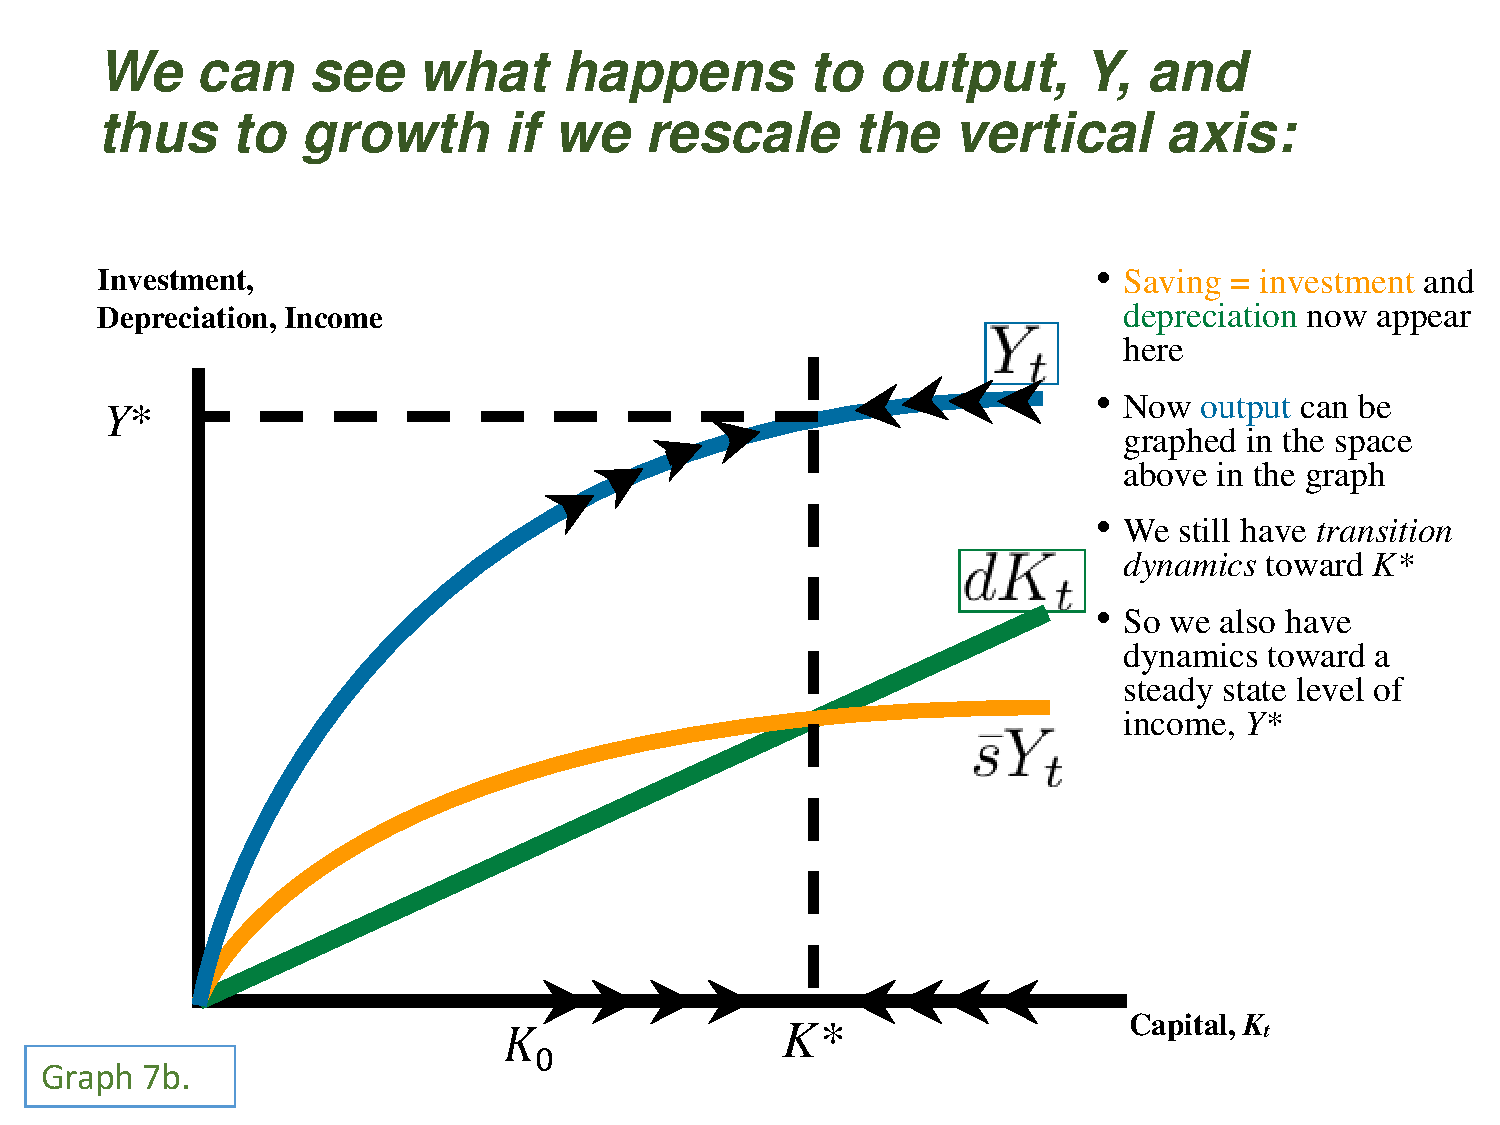
\includegraphics[width=.3\textwidth]{solow_graph}

\subsubsection{Solving for steady state}
At steady state, investment = depreciation

\begin{tabulary}{\linewidth}{ll}
	$\bar s Y^*$ 	& $= \bar d K^*$\\
				& $= \bar s \bar A {K^*}^\alpha \bar L^{1-\alpha}$\\
	$\Rightarrow K^*$		& $=\bar L {(\frac{\bar s \bar A}{\bar d})}^{\frac{1}{1-\alpha}}$\\
	\ \\
	$\Rightarrow Y^*$		& $=\bar A {K^*}^\alpha \bar L^{1-\alpha}$\\
						& $=\bar A^{\frac{1}{1-\alpha}}(\frac{\bar s}{\bar d})^{\frac{\alpha}{1-\alpha}}\bar L$
\end{tabulary}

\subsubsection{Note}
population ($\bar L$) growth can increase aggregate output ($Y^*$) but not output per capita ($y^*$)\\
$g_y = g_Y - g_L = 0$

\subsubsection{Transition Dynamics}
Explains the different growth rate:\\
below steady state $\rightarrow$ grow\\
above steady state $\rightarrow$ negative growth

\subsubsection{Strength and weakness}
\begin{tabulary}{\linewidth}{lL}
	strength:   &	1. explains steady state\\
			&	2. has principal of transition dynamics\\
	
	weakness: &	1. focus only on investment can capital (TFP unexplained)\\
			&	2. no explanation for different investment and productivity rates\\
			&	3. no explanation for sustained long-run economic growth
\end{tabulary}

\subsection{Romer model}
sustained economic growth due to the growth of new ideas ($A_t$)

Increasing then constant Return to Scale\\
$Y = \frac{X-\bar F}{10} \Rightarrow \frac{Y}{X} = \frac{1-\frac{\bar F}{X}}{10}$\\
where $X := $ production, $\bar F :=$ fixed cost
\ \\
\ \\
4 equations
\begin{tabulary}{\linewidth}{lL}
	Output production function:	&	$Y_t = A_t L_{yt}$\\
	Idea production function: &			$\Delta A_{t+1} = \bar z A_t L_{at}$\\
	Resource constraint: &			$L_{yt} + L_{at} = \bar L$\\
	Allocation of labour: &		$L_{at} = \bar l \bar L$
\end{tabulary}

\ \\
4 variables
\begin{tabulary}{\linewidth}{llll}
	$Y_t$:	&				output at time t & $A_t$: &				ideas at time t\\
	$L_{yt}$: 	&				labour for output, time t & $L_{at}$: &	researchers at time t\\
\end{tabulary}

\ \\
4 parameters
\begin{tabulary}{\linewidth}{ll}
	$\bar z$:		&	research productivity\\
	$\bar L$:		&	total labour force\\
	$\bar l$:		&	proportion of research labour\\
	$\bar A_0$:	&	initial pool of ideas
\end{tabulary}

\subsubsection{Solution}
\begin{tabulary}{\linewidth}{lL}
	$y_t := \frac{Y_t}{\bar L}$ &			$= A_t(1-\bar l)$\\
	$g_A = \frac{\Delta A_{t+1}}{A_t}$&	$= \bar z L_{at} = \bar z \bar l \bar L$\\
	$A_t =$ &				$\bar A_0 (1+\bar g_A)^t$ (stock of knowledge)\\
	$y_t =$ &			$\bar A_0 (1-\bar l)(1+\bar g_A)^t$
\end{tabulary}

\subsubsection{If diminishing return to idea}
\begin{tabulary}{\linewidth}{ll}
	constant return to idea: & $\Delta A_{t+1} = \bar z A_t L_{at}$\\
	diminishing return to idea: & $\Delta A_{t+1} = \bar z A_t ^\alpha L_{at}$
\end{tabulary}

there will still be sustained growth, but growth effect are eliminated due to diminishing returns

\subsection{Combining Solow and Romer models}
Explains the different growth rate (instead of constant growth rate as proposed in Romer model)\\
Exhibits transition dynamics if economy is not on its balanced growth path
\begin{tabulary}{\linewidth}{ll}
	short period:	&	countries have different growth rate\\
	long period:	&	countries grow at the same rate
\end{tabulary}

\subsubsection{Growth accounting}
determine the sources of growth in an economy and how they changes over time\\
$Y_t = A_t K_t^{1/3} L_{yt}^{2/3} \Rightarrow g_{Y_t} = g_{A_t} + \frac{1}{3}g_{K_t} + \frac{2}{3} g_{L_{yt}}$

adjust for labour hours
$g_{Y_t} - g_{L_t} = \frac{1}{3}(g_{K_t} - g_{L_t}) + \frac{2}{3} (g_{L_{yt}} - g_{L_t}) + g_{A_t}$

\subsubsection{Combining Solow and Romer Algebraically}

5 equations
\begin{tabulary}{\linewidth}{lL}
	Output production function:	&	$Y_t = A_tK_t^{1/3}L_{yt}^{2/3}$\\
	Capital production function: &		$\Delta K_{t+1} = \bar s Y_t - \bar d K_t$\\
	Idea production function: &		$\Delta A_{t+1} = \bar z A_t L_{at}$\\
	Resource constraint: &			$L_{yt} + L_{at} = \bar L$\\
	Allocation of labour: &			$L_{at} = \bar l \bar L$
\end{tabulary}

\ \\
4 variables
\begin{tabulary}{\linewidth}{llll}
	$Y_t$:	&				output at time t & $A_t$: &				ideas at time t\\
	$L_{yt}$: 	&				labour for output at time t & $L_{at}$: &	researchers at time t\\
\end{tabulary}

\ \\
5 parameters
\begin{tabulary}{\linewidth}{ll}
	$\bar z$:		&	research productivity\\
	$\bar L$:		&	total labour force\\
	$\bar l$:		&	proportion of research labour\\
	$\bar s$:		&	saving rate\\
	$\bar d$:		&	depreciation rate
\end{tabulary}

\subsubsection{Solution}
Production function now is:\\
constant return to scale in objects\\
increasing return to scale in ideas and objects together\\

At balanced growth path, $g_Y^*, g_K^*, g_A^*$ are constant

\ \\
$g_{Y_t} = g_{A_t} + \frac{1}{3}g_{K_t} + \frac{2}{3}g_{L_{yt}}$
\begin{tabulary}{\linewidth}{ll}
	$g_{K_t}$ & $= \frac{\Delta K_{t+1}}{K_t} = \bar s \frac{Y_t}{K_t} - \bar d$ = constant $\Rightarrow g_K^* = g_Y^*$\\
	$g_{A_t}$ & $= \bar z \bar l \bar L$\\
	$g_{L_{yt}}$ & $= 0$
\end{tabulary}
$\Rightarrow g_Y^* = \bar g_A + \frac{1}{3}g_Y^* \Rightarrow g_Y^* = \frac{3}{2}\bar g = \frac{3}{2}\bar z \bar l \bar L$\\
Higher growth rate than in Romer model due to growth in ideas

\ \\
per capita growth:\\
since $\frac{K^*_t}{Y_t^*} = \frac{\bar s}{g_y^* + \bar d} \Rightarrow y_t^* = (\frac{\bar s}{g_y^* + \bar d})^{1/2}{A_t^*}^{3/2}(1-\bar l)$

\end{multicols}
\end{document}